\documentclass[tikz]{standalone}
% A B C D E
% C A E B D
\begin{document}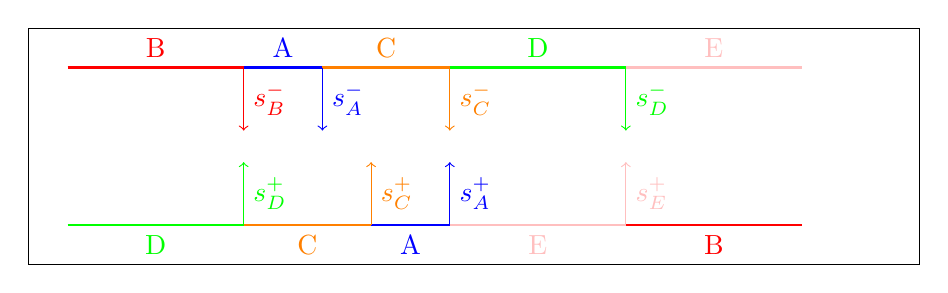
\begin{tikzpicture}
\draw (-.5, -1.5) rectangle (10.82,1.5);

\coordinate (t0) at (0,1);
\coordinate (t1) at (2.23606797749979, 1);
\coordinate (t2) at (3.23606797749979, 1);
\coordinate (t3) at (4.85410196624968, 1);
\coordinate (t4) at (7.09016994374947, 1);
\coordinate (t5) at (9.32623792124926, 1);

\coordinate (b0) at (0,-1);
\coordinate (b1) at (2.23606797749979, -1);
\coordinate (b2) at (3.85410196624968, -1);
\coordinate (b3) at (4.85410196624968, -1);
\coordinate (b4) at (7.09016994374947, -1);
\coordinate (b5) at (9.32623792124926, -1);

\draw[thick,red] (t0) -- node[above] {B} (t1);
\draw[thick,blue] (t1) -- node[above] {A} (t2);
\draw[thick,orange] (t2) -- node[above] {C} (t3);
\draw[thick,green] (t3) -- node[above] {D} (t4);
\draw[thick,pink] (t4) -- node[above] {E} (t5);

\draw[thick,green] (b0) -- node[below] {D} (b1);
\draw[thick,orange] (b1) -- node[below] {C} (b2);
\draw[thick,blue] (b2) -- node[below] {A} (b3);
\draw[thick,pink] (b3) -- node[below] {E} (b4);
\draw[thick,red] (b4) -- node[below] {B} (b5);

\draw[->,green] (b1) -- node[right] {$s^+_D$} +(0,0.8);
\draw[->,orange] (b2) -- node[right] {$s^+_C$} +(0,0.8);
\draw[->,blue] (b3) -- node[right] {$s^+_A$} +(0,0.8);
\draw[->,pink] (b4) -- node[right] {$s^+_E$} +(0,0.8);

\draw[->,red] (t1) -- node[right] {$s^-_B$} +(0,-0.8);
\draw[->,blue] (t2) -- node[right] {$s^-_A$} +(0,-0.8);
\draw[->,orange] (t3) -- node[right] {$s^-_C$} +(0,-0.8);
\draw[->,green] (t4) -- node[right] {$s^-_D$} +(0,-0.8);

\end{tikzpicture}\end{document}
